% User verification
% - Biometria twarzy
% - Ogólna procedura weryfikacji 
% - Przetwarzanie wstępne 
% - Neuronowy extractor cech
%   * Klasyfikacja
%   * Triplet loss
%       - Negative examples sampling
% - Implementacja


\section[verification]{System weryfikacji użytkownika za pomocą biometrii twarzy}\label{sec:verification}
\subsection{Komercyjne systemy weryfikacji twarzy}

\subsection{Procedura weryfikacji przy wykorzystaniu sieci neuronowych} 

Weryfikacja twarzy jest zadaniem przyrównania twarzy kandydata 
do innej i sprawdzenie czy nastąpiło ich dopasowanie. Jest to mapowanie
jeden-do-jednego: należy sprawdzić czy jest to ta sama osoba.

Mając na wejściu systemu dwa zdjęcia \(x_i\) oraz \(x_j\) wynik weryfikacji będzie wyznaczany następująco:

\begin{align}\label{eq:ekstraktor_weryfikacja}
\text{weryfikacja jest}\begin{cases}
    \text{pozytywna},& \text{jeśli } d(f(x_i), f(x_j) < \alpha \\
    \text{negatywna},              & \text{w.p.p}
\end{cases}
\end{align}

gdzie \(f(x)\) jest wektorem cech obrazu \(x\), opisanym w sekcji
\ref{sec:ekstraktor}, \(\alpha\) jest marginesem, \(d(f_1, f_2)\) jest pewną funkcją dystansu liczoną pomiędzy wektorami wyznaczanymi przez \(f(x)\).

\subsection{Wstępne przetwarzanie obrazu}
\subsubsection{Normalizacja obrazu}

\subsubsection{Normalizacja pozy}

\begin{figure}[H]
    \begin{center}
    \renewcommand\tabcolsep{1pt}
    {\bf Poprawna detekcja}
    \begin{tabular}{cc||cc||cc}
      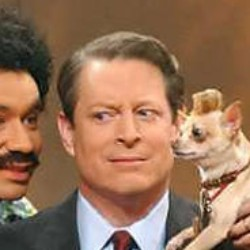
\includegraphics[width=.15\linewidth]{img/crop_examples/before/good/Al_Gore_0007.jpg} &
      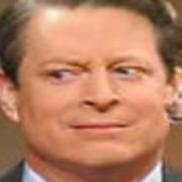
\includegraphics[width=.15\linewidth]{img/crop_examples/after/good/Al_Gore_0007.jpg} &
      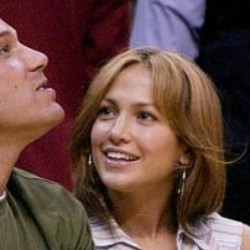
\includegraphics[width=.15\linewidth]{img/crop_examples/before/good/Jennifer_Lopez_0021.jpg} &
      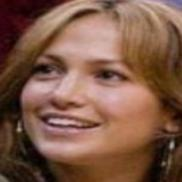
\includegraphics[width=.15\linewidth]{img/crop_examples/after/good/Jennifer_Lopez_0021.jpg} &
      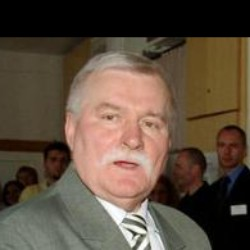
\includegraphics[width=.15\linewidth]{img/crop_examples/before/good/Lech_Walesa_0002.jpg} &
      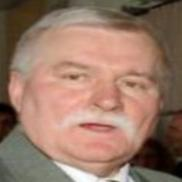
\includegraphics[width=.15\linewidth]{img/crop_examples/after/good/Lech_Walesa_0002.jpg} \\
    \end{tabular}
    {\bf Niepoprawna detekcja}
    \begin{tabular}{cc||cc||cc}
      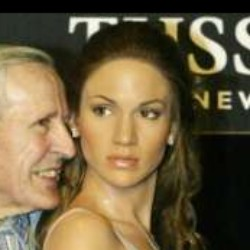
\includegraphics[width=.15\linewidth]{img/crop_examples/before/bad/Jennifer_Lopez_0020.jpg} &
      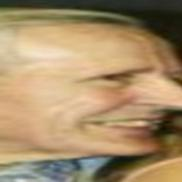
\includegraphics[width=.15\linewidth]{img/crop_examples/after/bad/Jennifer_Lopez_0020.jpg} &
      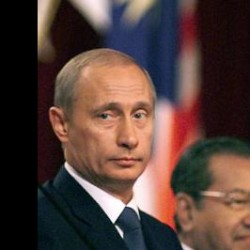
\includegraphics[width=.15\linewidth]{img/crop_examples/before/bad/Vladimir_Putin_0031.jpg} &
      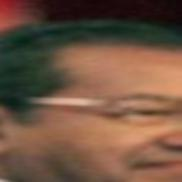
\includegraphics[width=.15\linewidth]{img/crop_examples/after/bad/Vladimir_Putin_0031.jpg} &
      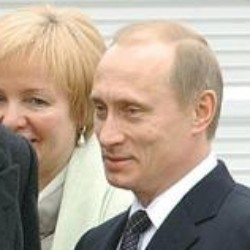
\includegraphics[width=.15\linewidth]{img/crop_examples/before/bad/Vladimir_Putin_0040.jpg} &
      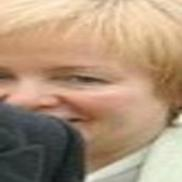
\includegraphics[width=.15\linewidth]{img/crop_examples/after/bad/Vladimir_Putin_0040.jpg} \\
    \end{tabular}
    \end{center}
    \caption{{\bf Przykłady działania ekstraktora twarzy.} Pokazane zostały tutaj wybrane przykłady prezentujące działanie ekstraktora twarzy.}
    \label{fig:ekstraktor_twarzy}
    \end{figure}

\subsection{Neuronowy ekstraktor cech} \label{sec:ekstraktor}
We współczesnych systemach weryfikacji wykorzystuje się głębokie sieci konwolucyjne. W
szczegółach zostaną omówione używana przez nas architektura w sekcji XXX. Pomijając szczegóły
modelu i traktując go jako czarną skrzynkę ogólna idea ekstraktora została pokazana na Rysunku
\ref{fig:ekstraktor_cech}. Głównym założeniem jest stworzenie systemu end-to-end, którego
rezultatem działania będzie embedding \(f(x)\), wyznaczony z obrazu wejściowego \(x\) przez
rzutowanie go do pewnej przestrzeni cech \(\mathbb{R}^d\), w taki sposób, że pewna funkcja
odległości wyznaczona dla wszystkich zdjęć twarzy jest mała dla twarzy należących do tych samych
osób i duża dla różnych twarzy. 

\begin{figure}[h]
    \centering
    \includegraphics[width=0.75\textwidth]{2-0_verification_ekstraktor_cech_drawio.pdf}
    \caption{\textbf{Struktura ekstraktora cech.} Ekstraktor składa się z wejścia, które w ogólnym przypadku może być paczką \(B\) przetworzonych wstępnie obrazów twarzy o wymiarach \( W \times H \times C\), głębokiej sieci konwolucyjnej i następującej po niej warstwie normalizacji. W rezultacie na wyjściu otrzymujemy \(B\) wektorów cech o wymiarach \(D\).}
    \label{fig:ekstraktor_cech}
\end{figure}


W literaturze można znaleźć dwie rodziny algorytmów trenujących, jedna wzorująca się na
klasycznym podejściu stosowanym podczas treningu klasyfikatorów obrazów. Najnowsze podejścia z
tej rodziny algorytmów prezentujemy w sekcji \ref{sec:klasyfikatory}. Drugi rodzaj algorytmów
bazują na optymalizacji multi-class classification hinge loss (po pl?). Opisujemy je w
szczegółach w sekcji \ref{sec:tripletloss}

\subsubsection{Klasyfikacja twarzy}\label{sec:klasyfikatory}
\begin{figure}[h!]
\centering
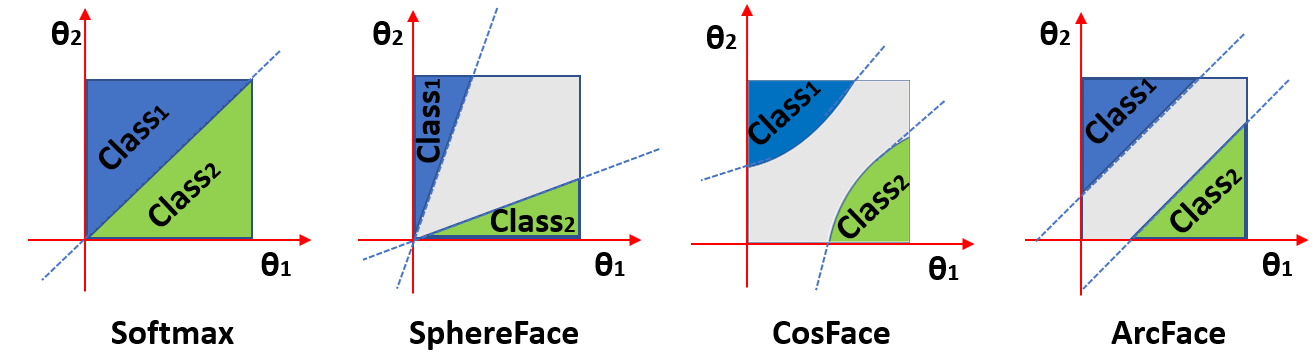
\includegraphics[width=1\linewidth]{img/margincompare.png}
\caption{Porównanie marginesów decyzyjnych\cite{}}
\vspace{-4mm}
\label{fig:binarymargin}
\end{figure}
\paragraph{Softmax\cite{Centreloss}}
\paragraph{SphereFace}
\paragraph{CosFace\cite{Cosface}}
\paragraph{ArcFace\cite{Arcface}}


\subsubsection{FaceNet}\label{sec:tripletloss}
% \begin{align}\label{eq:triplet_dystant}
    % \left\Vert f(x_i) - f(x_j) \right\Vert_q^p < \alpha
% \end{align}



